\secnumbersection{DEFINICIÓN DEL PROBLEMA}

Santiago posee uno de los sistemas de transporte público más masivos y avanzados de América Latina, caracterizado por la integración de buses, metro y tren suburbano. Según registros operativos oficiales, el sistema integrado supera las siete millones de transacciones en un día laboral promedio, de las cuales 5,0 millones corresponden exclusivamente a la red de buses \cite{dtpm_informe_2025}. La red de movilidad de la ciudad conecta a una población metropolitana que supera los siete millones de habitantes, distribuida en más de cuarenta comunas.

Comprender la distribución espacial de los desplazamientos en esta red, representada mediante flujos origen-destino (OD), es un insumo esencial para la planificación del transporte. También lo es para el diseño de infraestructura vial y la formulación de políticas urbanas basadas en evidencia \cite{liu2024interdisciplinary}.

\subsection{Fuentes de datos actuales y sus limitaciones}

La planificación del transporte en Santiago se apoya actualmente en dos fuentes principales de datos de movilidad. La primera es la \textit{Encuesta Origen-Destino} (EOD) de SECTRA\footnote{Secretaría de Planificación del Transporte, organismo dependiente del Ministerio de Transportes y Telecomunicaciones de Chile.}. Su última versión fue levantada en 2012, con actualizaciones parciales en 2017. Esta encuesta constituye la referencia canónica de flujos de movilidad en la ciudad. Sin embargo, su periodicidad de siete a diez años implica que los datos disponibles pueden no reflejar la movilidad actual. Esto es especialmente relevante tras la reconfiguración de patrones de desplazamiento producida por la pandemia de COVID-19. Su elevado costo de levantamiento agrava además esta desactualización.

La segunda fuente son los datos anonimizados de validación de la \textit{tarjeta bip!}\footnote{Nombre oficial del sistema de tarificación electrónica del transporte público de Santiago.}, administrados por el DTPM\footnote{Directorio de Transporte Público Metropolitano.}. Estos datos registran validaciones en Metro y buses con alta resolución temporal. No obstante, no cubren etapas caminadas. Tampoco cubren viajes en taxi o colectivo pagados en efectivo, ni modos no motorizados.

Esta brecha entre la necesidad de datos actualizados y su disponibilidad real motiva el desarrollo de modelos generativos. Dichos modelos deben ser capaces de estimar flujos OD a partir de características observables del territorio, sin depender exclusivamente de encuestas o registros transaccionales.

\subsection{Limitaciones de los modelos vigentes}

Los modelos utilizados en la práctica para la estimación de flujos en Santiago corresponden a modelos de gravedad clásicos. Estos modelos presentan limitaciones ampliamente documentadas en la literatura \cite{simini2012universal, liu2024interdisciplinary}. Imponen relaciones paramétricas monótonas entre población, distancia y flujo, lo que genera un ajuste deficiente ante fenómenos no lineales, como la existencia de subcentros de empleo o corredores de transporte masivo. Requieren además calibración manual para cada contexto geográfico, lo que limita su transferibilidad. Finalmente, no incorporan como variables explicativas el tejido urbano: puntos de interés, uso de suelo ni infraestructura de transporte.

Modelos basados en aprendizaje profundo, como Deep Gravity \cite{simini2021deep}, han demostrado superar estas limitaciones incorporando variables geoespaciales de OpenStreetMap. Su arquitectura y su desempeño reportado se detallan en el Marco Conceptual de esta memoria. Sin embargo, su aplicación en ciudades latinoamericanas no ha sido explorada.

\subsection{Especificidad del contexto latinoamericano}

Esta ausencia de validación es relevante porque las ciudades latinoamericanas presentan características estructurales que las diferencian de los contextos donde estos modelos han sido desarrollados y evaluados. La segregación socio-espacial severa, la existencia de periferias urbanas de bajos ingresos con infraestructura de transporte deficitaria y la coexistencia de sistemas formales e informales de movilidad generan patrones de desplazamiento que no responden a las funciones de disuasión por distancia calibradas en ciudades del Norte Global \cite{vecchio2020transport}. A esto se suma la heterogeneidad en la completitud de los datos geoespaciales abiertos: estudios recientes demuestran que la cobertura de OpenStreetMap en ciudades latinoamericanas alcanza apenas un 10 a 20\% en datos de edificaciones, frente a más del 50\% en Europa y Norteamérica, con un sesgo intra-ciudad correlacionado con el nivel de desarrollo humano subnacional \cite{herfort2023spatio, BarringtonLeigh2017}.

En el caso específico de Santiago, evidencia empírica reciente basada en datos de telefonía móvil y enrutamiento multimodal demuestra que la proximidad espacial no se traduce en accesibilidad equitativa \cite{marinflores2026proximity}. Las poblaciones periféricas de menores ingresos enfrentan penalizaciones estructurales de accesibilidad y un conjunto restringido de opciones de destino, lo que implica que modelos que asumen un comportamiento uniforme de proximidad-a-oportunidad generarán predicciones sesgadas en este contexto. Esta dinámica contrasta con las ciudades europeas y norteamericanas donde \textit{Deep Gravity} fue validado, donde la distribución de oportunidades urbanas es comparativamente más homogénea.

Más allá del contexto geográfico, el modelo carece de una capa de explicabilidad que permita a los planificadores comprender qué factores del tejido urbano impulsan cada predicción. Esta carencia es especialmente crítica en el contexto latinoamericano, donde la auditoría de las predicciones es un requisito para fundamentar inversiones públicas en un escenario de recursos limitados.

\subsection{Síntesis del problema}

En síntesis, el problema que aborda esta memoria se formula de la siguiente manera:

\begin{quote}
\textit{La planificación del transporte en Santiago de Chile opera con estimaciones de flujos OD basadas en datos desactualizados y modelos paramétricos que no capturan la complejidad del tejido urbano. Modelos basados en aprendizaje profundo, como Deep Gravity, han demostrado superar estas limitaciones, pero su aplicación en ciudades latinoamericanas no ha sido explorada. Se desconoce tanto su capacidad predictiva en este contexto como la contribución de las amenities urbanas a la generación de flujos. Asimismo, la ausencia de técnicas de explicabilidad sobre estos modelos impide que los planificadores comprendan los factores que determinan las predicciones.}
\end{quote}

\clearpage
\subsection{Árbol del problema}

A continuación se presenta el diagrama del árbol del problema (Figura \ref{fig:arbol_problema}):

\begin{figure}[H]
	\centering
	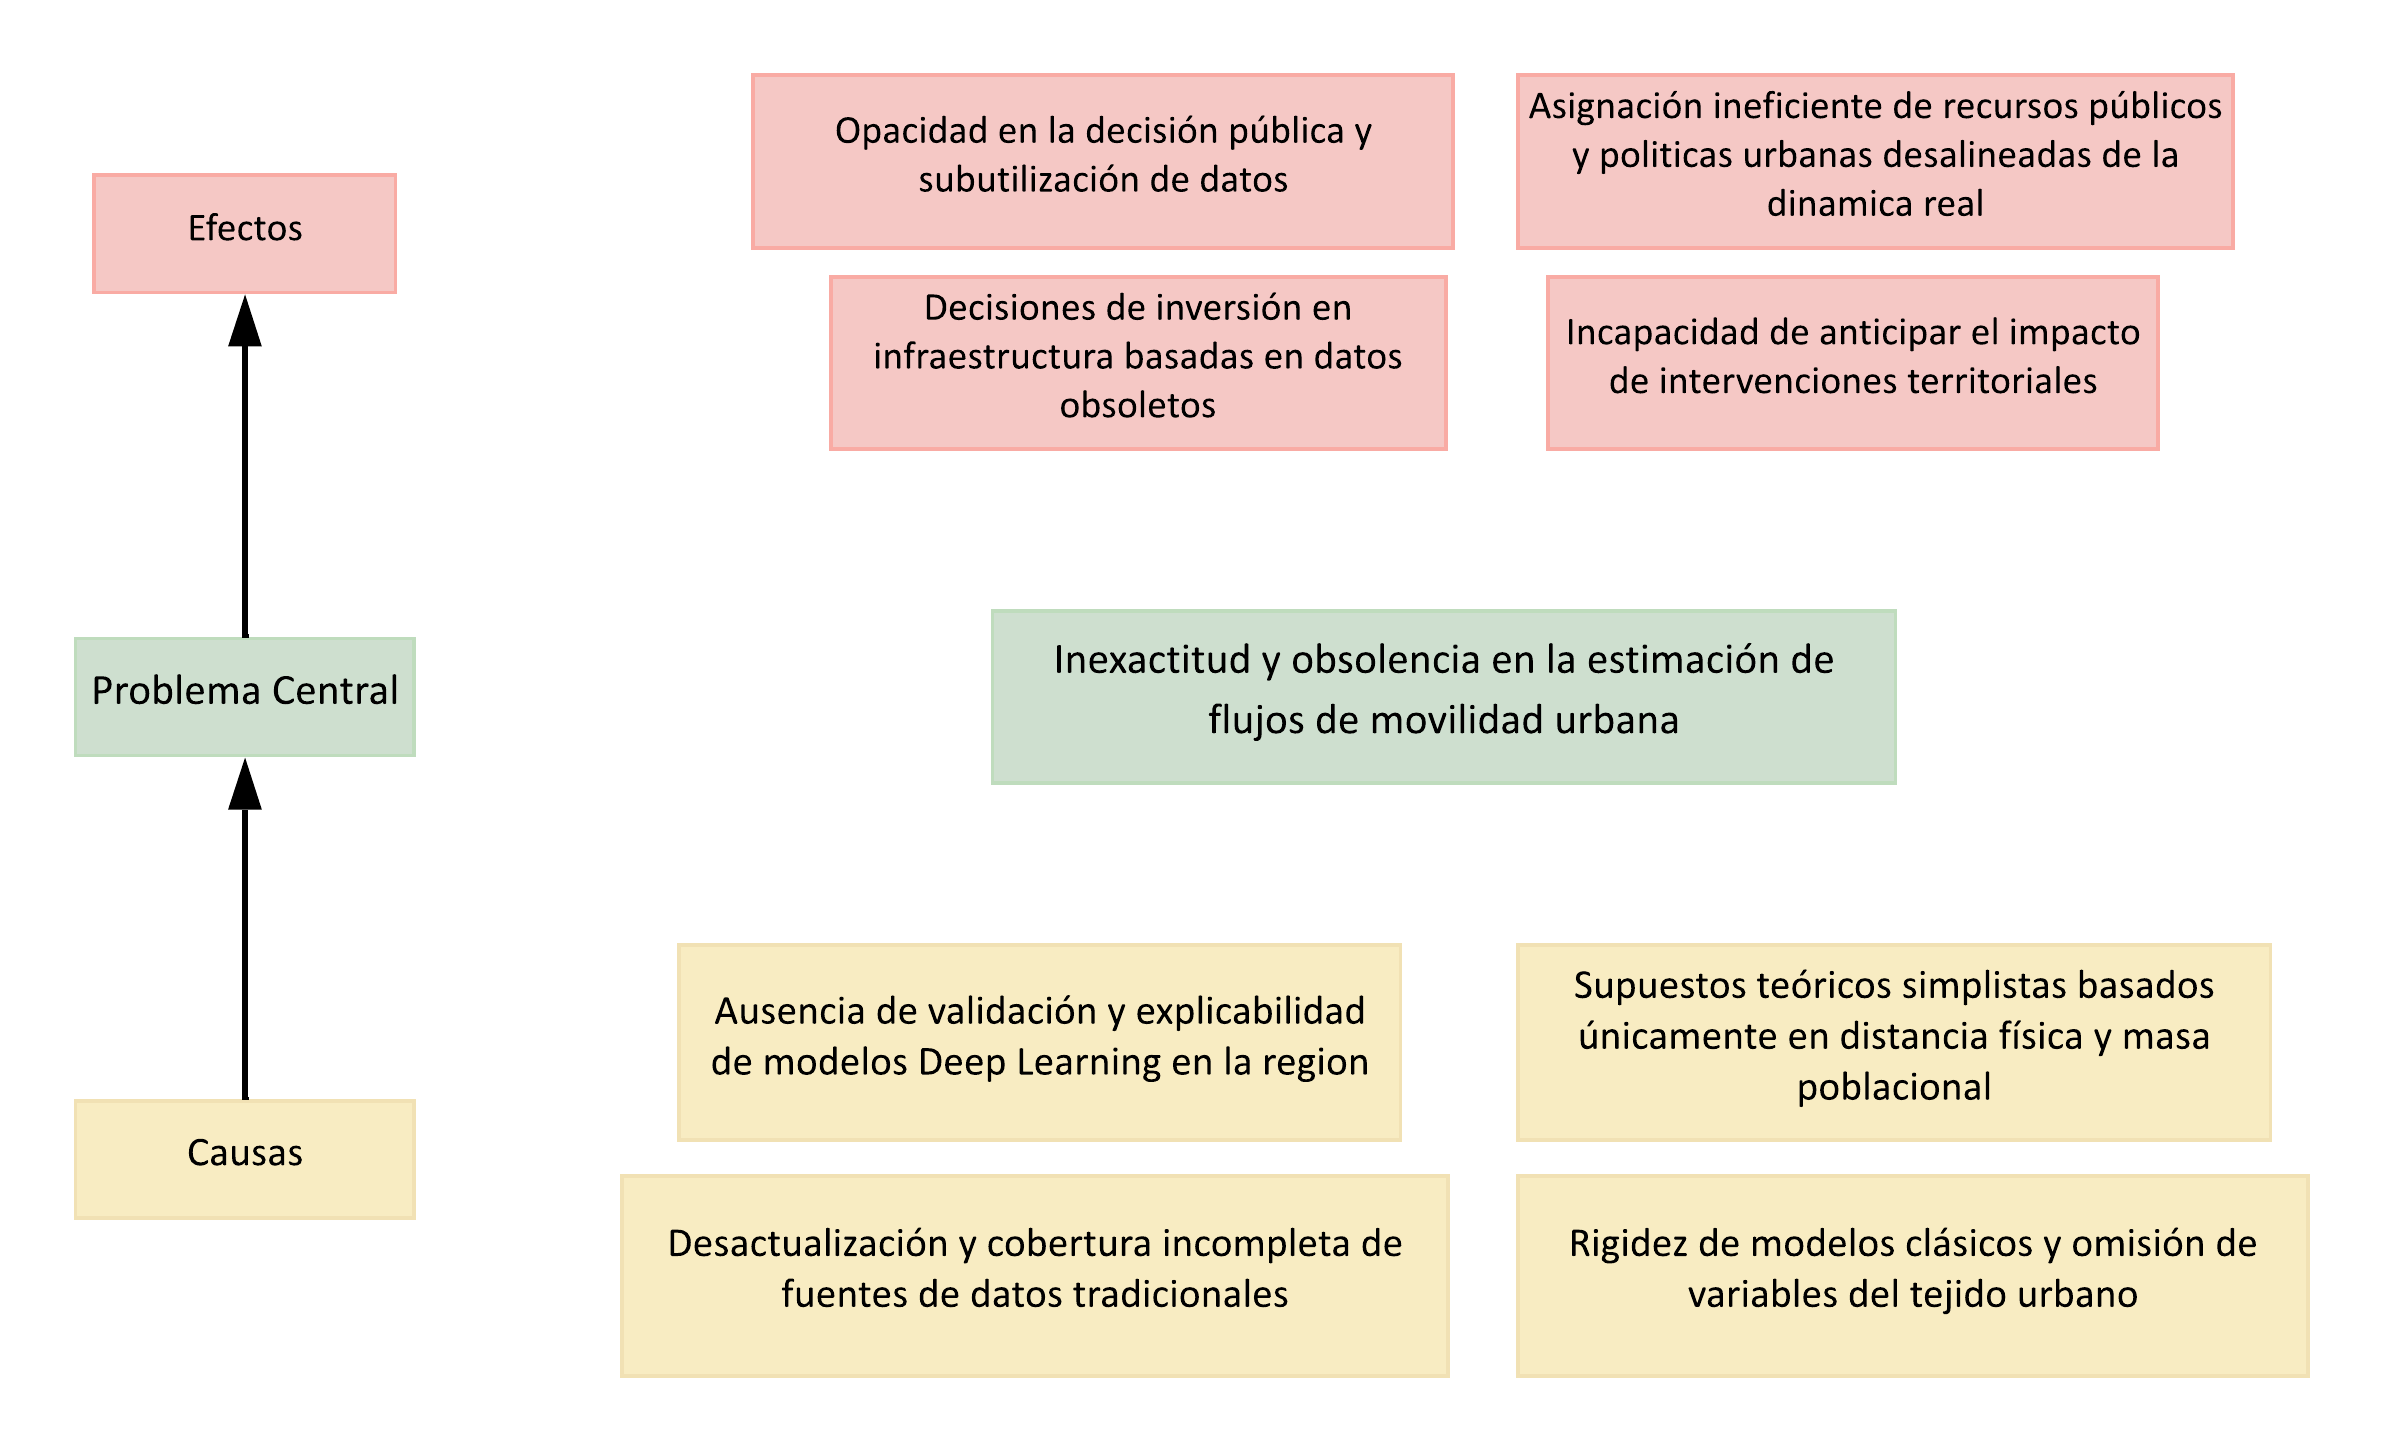
\includegraphics[width=\textwidth]{figures/arbol_del_problema.png}
	\caption{Diagrama del árbol del problema. Fuente: Elaboración propia.}
	\label{fig:arbol_problema}
\end{figure}

La Figura \ref{fig:arbol_problema} presenta el árbol del problema que resume los principales desafíos asociados a la estimación de movilidad en el Gran Santiago. En el centro se sitúa el problema fundamental: la inexactitud y obsolescencia en la estimación de flujos de movilidad urbana.

Este problema se origina por cuatro causas principales: la desactualización y cobertura incompleta de fuentes de datos tradicionales (EOD y bip!), la rigidez de los modelos gravitacionales clásicos al omitir variables del tejido urbano, los supuestos teóricos simplistas basados únicamente en distancia y masa poblacional, y la falta de validación y explicabilidad de modelos de Deep Learning en el contexto regional.

Como consecuencia, se generan cuatro efectos críticos: decisiones de inversión en infraestructura basadas en datos obsoletos, la incapacidad de anticipar el impacto de intervenciones territoriales, la opacidad en la decisión pública junto a la subutilización de datos masivos y abiertos, y una asignación ineficiente de recursos públicos con políticas desalineadas de la dinámica urbana real.

\subsection{Objetivo General}

Evaluar la sensibilidad de \textit{Deep Gravity} y de sus \textit{baselines} frente a la discretización espacial Zona 777--H3, a partir de una cohorte DTPM común, trazable y reproducible para Santiago de Chile.

\subsection{Objetivos Específicos}

\begin{enumerate}
	\item Auditar y adaptar el código de referencia, verificando contrato de datos, soporte de destinos, métrica CPC, caché y trazabilidad de ejecuciones, sin equiparar la auditoría técnica de Nueva York con una reproducción científica integral.

	\item Reconstruir viajes canónicos desde las tablas DTPM de viajes y etapas, definir una cohorte común y delimitar el núcleo urbano de Santiago mediante reglas espaciales reproducibles.

	\item Construir adaptadores comparables para Zona 777 y H3, evaluar la factibilidad de H3-r3 a H3-r8 y conservar Zona 777, H3-r7 y H3-r8 como representaciones candidatas sujetas a validación.

	\item Construir atributos de población y OSM con fuentes, unidades, reglas de agregación y normalización explícitas, sin confundir población censal con generación observada.

	\item Entrenar y evaluar \textit{Deep Gravity} frente a distribuciones uniforme, de atracción de entrenamiento y de gravedad exponencial, usando CPC y particiones espaciales por \textit{tile} sobre un soporte de destinos común dentro de cada rama.

	\item Aplicar XAI solo al modelo final estabilizado, reportando su configuración y estabilidad, y sin interpretar las atribuciones predictivas como efectos causales.
	
\end{enumerate}
